\twocolumn[
\begin{center}
\title{\color[cmyk]{1, 0.57, 0, 0.38}{\Huge\bfseries Il Kernel Fedora \\}} % definisco il titolo dell'articolo
\author{\scriptsize Giuseppe Delvecchio (virus@fedoraonline.it)} % definisco l'autore e altre informazioni
\date{}
\end{center}
{\color[cmyk]{1, 0.46, 0, 0}\LARGE (Parte prima) Kernel - introduzione}\\
\maketitle
\normalsize
\doublespacing
\hfill
]
\onehalfspacing
\lettrine[lines=1, loversize=0.1, lraise=0.1]{\color[cmyk]{0.5, 0, 1, 0}\bfseries I}{}l giorno 15 agosto 1991 – Linus Torvalds scrive :
{\itshape “Sto programmando un sistema operativo (gratuito e solo per hobby, non vuole essere grande e professionale come GNU) per cloni di AT 386\ (486). È in preparazione da Aprile, e sta iniziando a funzionare...''}\\

Questa data può essere considerata la data di nascita del kernel linux.\\

\begin{figure}[!htbp]
\centering
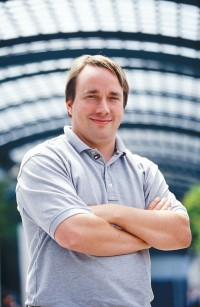
\includegraphics[scale=.40]{articoli/sistema_avanzato/immagini/torvalds.jpeg}
\caption{Linus Torvalds}
\end{figure}

Cosa è un kernel?\\

Esso è il nucleo software fondante di un sistema e fornisce tutte le funzioni essenziali per la gestione e il funzionamento del sistema.\\
Gestisce la memoria, la cpu, l'Input/Output, la rete, i filesystem, i dispositivi periferici, i processi ad essi collegati, le comunicazioni tra processi, le priorità di quest'ultimi, e molto altro ancora.\\

Tutto questo è solitamente trasparente all'utente medio che non si accorge di (quasi) nulla.\\

\begin{figure}[!htbp]
\centering

\includegraphics[scale=.20]{articoli/sistema_avanzato/immagini/tux.jpg}
\caption{Tux}
\end{figure}

Uno dei primi problemi che Linus ha dovuto affrontare è stata la scelta del tipo di kernel da costruire.
Egli costruì un kernel monolitico ovvero un kernel che sia un blocco di codice unico omnicomprensivo; ben presto però questo tipo di approccio rivelò i propri limiti, in quanto le dimensioni del kernel diventavano sempre più grandi (troppo) e il suo sviluppo complicato da gestire. La soluzione fu trovata usando un metodo diverso.\\

Pur mantenendo la struttura monolitica, furono creati moduli kernel che potessero essere caricati nel sistema in funzione delle esigenze, questi moduli che gestiscono determinati dispositivi, processi, filesystem, possono essere inclusi o meno nel kernel mediante opportuni comandi oppure inclusi in esso all'atto della compilazione.\\

Questo approccio è chiamato kernel modulare.\\

Quindi sostanzialmente il kernel attuale ha la possibilità di avere moduli interni che fanno blocco unico e/o vengono caricati al momento del boot anche in due momenti  successivi (kernel e initramfs), moduli caricabili successivamente al boot (operazione a cui provvede systemd oppure udev), e moduli che vengono totalmente esclusi, quindi mai caricabili a meno di non ricompilare il kernel.\\

I kernel rilasciati dalle varie distribuzioni linux differiscono proprio, anche se non esclusivamente, in questo; ognuna di esse ha fatto delle scelte precise di cosa inserire nel blocco unico, cosa rendere modulo caricabile, cosa escludere.\\

Spieghiamo brevemente il significato delle sigle presenti nel nome di un pacchetto rpm del kernel installato su fedora, prendendo per esempio il {\itshape kernel-PAE-3.1.9-4.fc16.i686}:

\begin{itemize}
\item la sigla PAE indica che si tratta di un kernel che supporta l'estensione dell'indirizzo fisico per la memoria, ovvero è in grado di rilevare ed utilizzare una ram maggiore di 4 Gb, questa versione PAE esiste solo per la 32 bit, ovviamente.
\item 3.1.9 – è la nuova numerazione semplificata introdotta da Linus Torvalds il 29 maggio 2011 in occasione del ventesimo anniversario del kernel linux:
\begin{itemize}
\item 3 --- è la major version che corrisponde alla “vecchia” 2.6;
\item 1 --- enumera i nuovi rilasci;
\item 9 --- enumera i rilasci di aggiornamenti di sicurezza e bug fix sul rilascio precedente;
\item 4 --- dopo il trattino seguono valori numerici tipici dei kernel compilati con patch oppure bug fix specifici introdotti dagli sviluppatori kernel della nostra fedora.
\item fc16 --- indica per quale versione fedora è stato rilasciato
\item i686 --- indica l'architettura del kernel, si tratta di una 32 bit sesta generazione delle cpu x86 intel e compatibili.
\end{itemize}
\end{itemize}

Una descrizione grafica di un kernel potrebbe essere la seguente:
{\itshape http://www.\ makelinux.net/kernel\_map/}.\\

\begin{figure*}[!t]
\centering
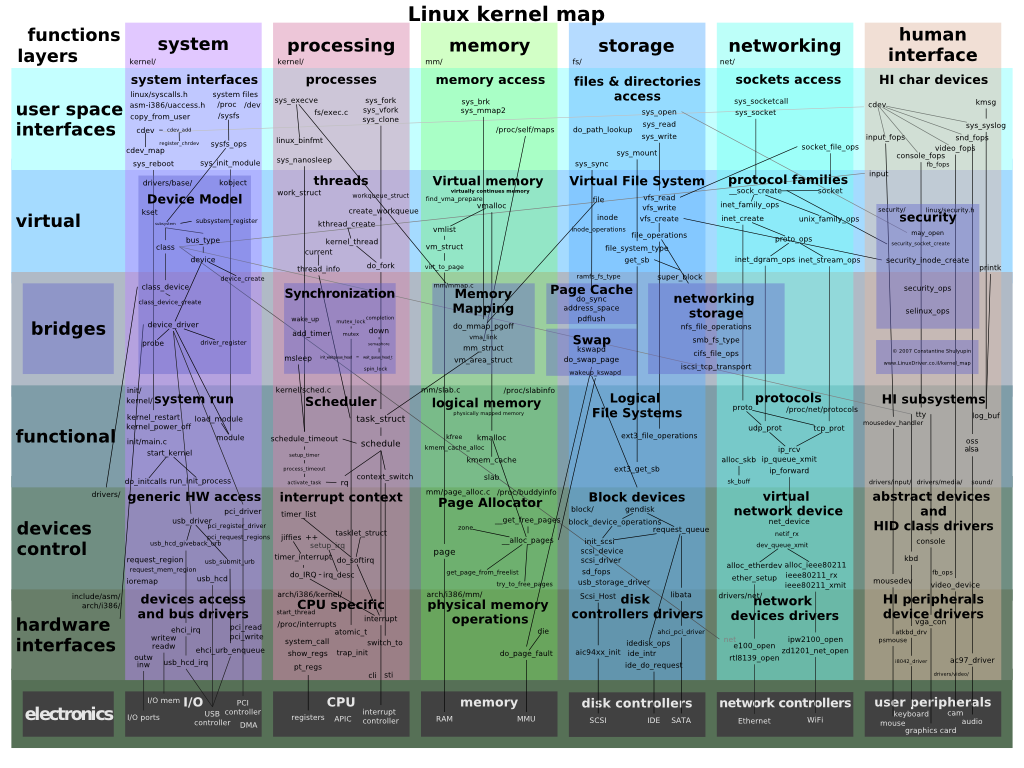
\includegraphics[scale=.40]{articoli/sistema_avanzato/immagini/kernel_map.png}
\caption{mappa del kernel ({\scriptsize fonte: http://it.wikipedia.org/})}
\end{figure*}

La grande complessità di questa mappa ci spaventa ma ci fa rendere conto del lavoro che è stato eseguito per costruire un kernel.\\

Quando è necessario compilare un kernel?

\begin{enumerate}
\item  per far funzionare un componente particolare che non è gestito dal kernel che si utilizza, il cui modulo esiste ma non è stato incluso;
\item per utilizzare l'ultima versione kernel se non è disponibile il pacchetto precompilato;
\item per fare test “particolari” al proprio sistema;
\item a scopi “didattici''.
\end{enumerate}

\hfill {\itshape (fine prima parte)}
